\section{Mathematische Grundlagen}
\subsection{Vektorfelder}
\subsubsection{Divergenz}
	Die Divergenz beschreibt die Quellendichte eines Skalarfeldes. 
	Interpretiert man ein Vektorfeld als Strömungsfeld, so gibt die Divergenz für jede
	Stelle die Tendenz an, ob ein Teilchen in der Nähe zu diesem Punkt hin- bzw.
	von diesem Punkt wegfliesst. Es sagt damit aus, ob und wo das Vektorfeld Quellen
	(Divergenz grösser als Null) oder Senken (Divergenz kleiner als Null) hat. Ist
	die Divergenz überall gleich Null, so bezeichnet man das Feld als quellenfrei.\\
	
	$\boxed{\divergenz \vec{F}=\nabla \cdot \vec{F}= \frac{\partial F}{\partial x}+\frac{\partial F}{\partial y}+\frac{\partial F}{\partial z}}$

\subsubsection{Rotation}
Interpretiert man ein Vektorfeld als Strömungsfeld, so gibt die Rotation für jeden
Ort an, wie schnell und um welche Achse ein mitschwimmender Körper rotieren
würde. Ein Vektorfeld, dessen Rotation überall null ist, nennt man wirbelfrei.\\

$\boxed{\rotation(\vec F)=\nabla\times\vec{F} = 
	\begin{pmatrix}
	(F_3)_y - (F_2)_z\\
	(F_1)_z - (F_3)_x\\
	(F_2)_x - (F_1)_y
	\end{pmatrix} = \left({\frac {\partial F_{z}}{\partial y}}-{\frac {\partial F_{y}}{\partial z}}\right){\hat {e}}_{x}+\left({\frac {\partial F_{x}}{\partial z}}-{\frac {\partial F_{z}}{\partial x}}\right){\hat {e}}_{y}+\left({\frac {\partial F_{y}}{\partial x}}-{\frac {\partial F_{x}}{\partial y}}\right){\hat {e}}_{z} \quad 
	\det
	\begin{vmatrix}
	e_x & e_y&e_z\\
	\dfrac{\partial}{\partial x} & \dfrac{\partial}{\partial x}& \dfrac{\partial}{\partial x}\\
	F_x& F_y & F_z
	\end{vmatrix}}$

\subsubsection{Gradient}
Der Gradient zeigt in einem Vektorfeld immer in die Richtung des steilsten Anstiegs. \\

$\boxed{\gradient(f)= \nabla \cdot f= 	
	\begin{pmatrix}
	\frac{\partial f}{\partial x}\\
	\frac{\partial f}{\partial y}\\
	\frac{\partial f}{\partial z}
	\end{pmatrix} ={\frac {\partial f}{\partial x}}{\hat {e}}_{x}+{\frac {\partial f}{\partial y}}{\hat {e}}_{y}+{\frac {\partial f}{\partial z}}{\hat {e}}_{z} }$

\subsubsection{Vektorpotential}
Das Vektorpotential A(r) ist eine Hilfsgrösse um den Umgang mit der magnetischen Flussdichte B(r) zu vereinfachen. \\
	$\boxed{\begin{matrix}
		B=\mu H\\
		B=\rotation A\\
		\varphi=\oint\limits_{C}A dr
		\end{matrix}}$

\subsubsection{Vektorfeldoperatoren}
\begin{tabular}{ll}
	\textbf{Nabla-Operator $\nabla$} & \textbf{Laplace-Operator $\Delta$}\\
	Operator um kontextabhängig & Operator um einem Skalarfeld\\
	Divergenz, Rotation oder Gradient darzustellen  &  die Divergenz seines Gradienten zuzuordnen\\
	$\nabla F=\frac{\partial F}{\partial x}+\frac{\partial F}{\partial y}+\frac{\partial F}{\partial z}$&$\Delta F=\frac{\partial^{2}F}{\partial x^{2}F}+\frac{\partial^{2}F}{\partial y^{2}}+\frac{\partial^{2}}{\partial z^{2}}$\\
	&$\Delta \vec{F} = \divergenz(\gradient(\vec{F}))$\\
	&$\Delta \vec{F} = \nabla \cdot (\nabla \cdot \vec{F})$\\	 
\end{tabular}
\subsubsection{Rechenregeln}
\begin{itemize}
	\item $\rotation(\gradient f) = 0 \qquad $ ``Gradientenfeld ist wirbelfrei''
	\item $\divergenz(\rotation \vec{v}) = 0 \qquad $ ``Feld der Rotation ist quellenfrei''
	\item $\divergenz(f\vec{v}) = (\gradient f) \cdot \vec{v} + f \divergenz \vec{v}$
	\item $\rotation(f\vec{v}) = (\gradient f) \times \vec{v} + f \rotation \vec{v}$
	\item $\rotation(\rotation \vec{v}) = \gradient(\divergenz \vec{v}) - \Delta \vec{v}$
\end{itemize}
\subsubsection{Laplace-Operator Koordinatentranfsormation}
\begin{itemize}
	\item Laplace-Operator in kartesischen Koordinaten
	\[\Delta U(x,y,z) = \frac{\partial^{2}}{\partial x^{2}}+\frac{\partial^{2}}{\partial y^{2}}+\frac{\partial^{2}}{\partial z^{2}}\]
	\item Laplace-Operator in Zylinderkoordinaten
	\[\Delta U(r,\alpha,z) = \frac{1}{r} \dfrac{\partial}{\partial r} \left(r \frac{\partial U}{\partial r}\right) + \frac{1}{r^2}\frac{\partial^2 U}{\partial \alpha^2}+\dfrac{\partial^2 U}{\partial z^2} \]
	\item Laplace-Operator in Kugelkoordinaten
	\[\Delta U(r,\vartheta,\varphi) = \frac{1}{r^2} \dfrac{\partial}{\partial r} \left( r^2 \frac{\partial U}{\partial r}\right) + \frac{1}{r^2 \sin(\vartheta)}\frac{\partial}{\partial \vartheta}\left(sin(\vartheta)\dfrac{\partial U}{\partial \vartheta} \right) +\frac{1}{r^2 sin^2(\vartheta)}\dfrac{\partial^2 U}{\partial \varphi^2}\]
\end{itemize}
\subsection{Differentialrechnung}
\subsubsection{Ableitungsregeln}
\renewcommand{\arraystretch}{1.5}
\begin{tabular}{|l|l|}
	\hline \textbf{Konstantenregeln}& $c'=0'$\\
	\hline \textbf{Faktorenregeln}& $(cu)'=c u'$\\
	\hline \textbf{Summenregel}& $(u\pm v)'= u' \pm v'$\\
	\hline \textbf{Produktregel}& $(uv)'=u'v + uv'$\\
	\hline \textbf{Quotientenregel}& $(\frac{u}{v})'= \frac{u'v-uv'}{u^{2}}$\\
	\hline \textbf{Kettenregel}& $y=u(v(x)) ; y'=\frac{du}{dv} \frac{dv}{dx}$\\
	\hline \textbf{Potenzregel} & $(u^{a})'=au^{a-1}$\\
	& $(\frac{1}{u})'= \frac{u'}{u^2}$\\
	\hline	\textbf{Wurzelregel} & $f(x)=\sqrt{x} ; f'(x)=\frac{1}{2\sqrt{x}}$\\
	\hline	\textbf{Logarithmusregel} & $\ln{u}'=\frac{u'}{u}$\\ 
	\hline	\textbf{Differentation der Umkehrfunktion} & $(f^{-1})'(y)=\frac{1}{f'(x)} $\\
	\hline 
\end{tabular}
\subsubsection{Ableitung elementarer Funktionen}
\renewcommand{\arraystretch}{2.2}
\begin{tabular}{|l|l||l|l|}
	\hline
	\textbf{Funktion} & \textbf{Ableitung} & \textbf{Funktion} &
	\textbf{Ableitung}\\\hline
	\hline $C$ (Konstante) & 0 & $\sec x$ & $\dfrac{\sin x}{\cos^2 x}$ \\
	\hline $x$ & 1 & $\sec^{-1} x$ & $\dfrac{-\cos x}{\sin^2 x}$\\
	\hline $x^n$ ($n\in\mathbb{R}$) & $nx^{n-1}$ & $\arcsin x \quad (|x| < 1)$ &
	$\dfrac{1}{\sqrt{1-x^2}}$\\
	\hline $\dfrac{1}{x}$ & $-\dfrac{1}{x^2}$ & $\arccos x \quad (|x| < 1)$ &
	$-\dfrac{1}{\sqrt{1-x^2}}$\\
	\hline $\dfrac{1}{x^n}$ & $-\dfrac{n}{x^{n+1}}$ & $\arctan x$ & $\dfrac{1}{1+x^2}$\\
	\hline $\sqrt{x}$ & $\dfrac{1}{2\sqrt{x}}$ & $\arccot{x} $ & $-\dfrac{1}{1+x^2}$\\
	\hline $\sqrt[n]{x}\quad (n\in\mathbb{R}, n \neq 0, x > 0)$ &
	$\dfrac{1}{n\sqrt[n]{x^{n-1}}}$ & $\arcsec x$ & $\dfrac{1}{x\sqrt{x^2-1}}$\\
	\hline $\mathrm{e}^x$ & $\mathrm{e}^x$ & $\arcossec x$ & $-\dfrac{1}{x\sqrt{x^2-1}}$\\
	\hline $\mathrm{e}^{bx}\quad (b\in\mathbb{R})$ & $b\mathrm{e}^{bx}$ & $\sinh x$ &
	$\cosh x$\\
	\hline $a^x\quad (a > 0)$ & $a^x\ln a$ & $\cosh x$ & $\sinh x$\\
	\hline $a^{bx}\quad (b\in\mathbb{R}, a > 0)$ & $ba^{bx}\ln a$ & $\tanh x$ &
	$\dfrac{1}{\cosh^2 x}$\\
	\hline $\ln x$ & $\dfrac{1}{x}$ & $\coth x \quad(x \neq 0)$ & $-\dfrac{1}{\sinh^2 x}$\\
	\hline $\log_a{x} \quad (a > 0, a \neq 1, x > 0)$ &
	$\dfrac{1}{x}\log_a{\mathrm{e}}=\dfrac{1}{x\ln a}$ & $\arsinh x$ &
	$\dfrac{1}{\sqrt{1+x^2}}$\\
	\hline $\lg x \quad (x > 0)$ & $\dfrac{1}{x}\lg \mathrm{e}\approx \dfrac{0.4343}{x}$
	& $\arcosh x \quad (x > 1)$ & $\dfrac{1}{\sqrt{x^2-1}}$\\
	\hline $\sin x$ & $\cos x$ & $\artanh x \quad (|x| < 1)$ & $\dfrac{1}{1-x^2}$\\
	\hline $\cos x$ & $-\sin x$ & $\arcoth x \quad (|x| > 1)$ & $-\dfrac{1}{x^2-1}$\\
	\hline $\tan x \quad (x\neq(2k+1)\dfrac{\pi}{2}, k\in\mathbb{Z})$ & $\dfrac{1}{\cos^2
		x}=\sec^2 x$ & $[f(x)]^n \quad (n\in\mathbb{R})$ & $n[f(x)]^{n-1}f'(x)$\\
	\hline $\cot x \quad (x\neq k\pi, k\in\mathbb{Z})$ & $\dfrac{-1}{\sin^2 x}=-cosec^2x$ & $\ln f(x) \quad (f(x)> 0)$ & $\dfrac{f'(x)}{f(x)}$\\
	\hline
\end{tabular}
\clearpage
\pagebreak
\subsection{Lineare Differentialgleichung 2. Ordnung}
\renewcommand{\arraystretch}{1.2}
\begin{tabular}{p{8cm}p{8cm}}
	\textbf{Form:} $y''+a_1\cdot y'+a_0\cdot y=f(x)$  &
	\textbf{St"orglied:} $f(x)$\\
	\textbf{Homogene Differentialgleichung:} $f(x)=0$ &
	\textbf{Inhomogene Differentialgleichung:} $f(x)\neq 0$\\
	\textbf{Allgemeine Lösung einer DGL: }	$Y=y_H+y_P$& \\
\end{tabular}

\subsubsection{Homogene Lösung $y_H$}
\begin{tabular}{p{8cm}p{8cm}}
	\textbf{Charakteristisches Polynom:}\newline
	$\lambda^2+a_1\cdot\lambda+a_0=0$&	
	\textbf{Durch Mitternachtsformel lösen: }\newline
	$\lambda_{1,2}={\frac {-b\pm {\sqrt {b^{2}-4ac}}}{2a}}$\\
	\textbf{Diskriminante: }\newline
	$D = b^2-4ac $&\\
\end{tabular}

\begin{tabular}{|p{6cm}|p{8cm}|}
	\hline
	Falls $ \lambda_1\neq \lambda_2 \quad D > 0$&
	$y_H=A_1e^{\lambda_1x}+A_2e^{\lambda_2x}$\\
	\hline
	Falls $\lambda_1= \lambda_2 \quad D = 0$&
	$y_H=e^{\lambda_1x}(A_1+A_2\cdot x)$\\
	\hline
	Falls $\lambda_{1,2}= -\frac{a_1}{2} \pm jb \quad D < 0$&
	$y_H=e^{-\frac{1}{2}a_1x}(A \cdot cos(b) +B \cdot sin(b))$\\
	\hline
\end{tabular}

\subsubsection{Partikuläre Lösung $y_P$ durch Form des Störglieds $f(x)$}
\textbf{Allgemeines Vorgehen:}\\
1. Ermitteltes $y_P$ n mal ableiten \\
2. Ableitungen in DGL einsetzen \\
3. Koeffizientenvergleich \\
\vspace{0.2cm}\\
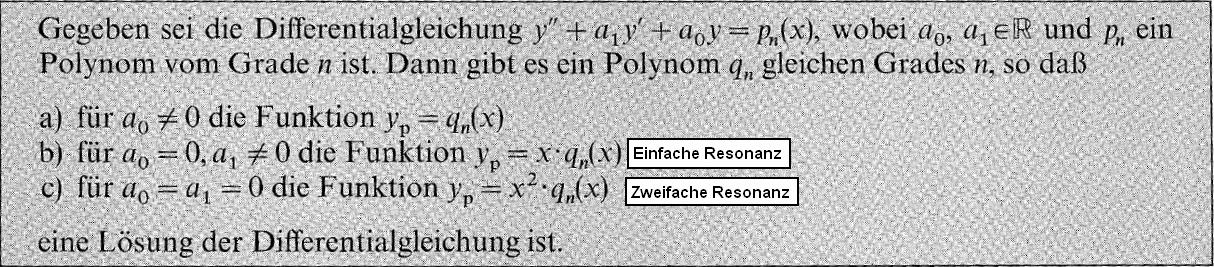
\includegraphics[width=\linewidth]{images/DGL_Part_1.jpg}
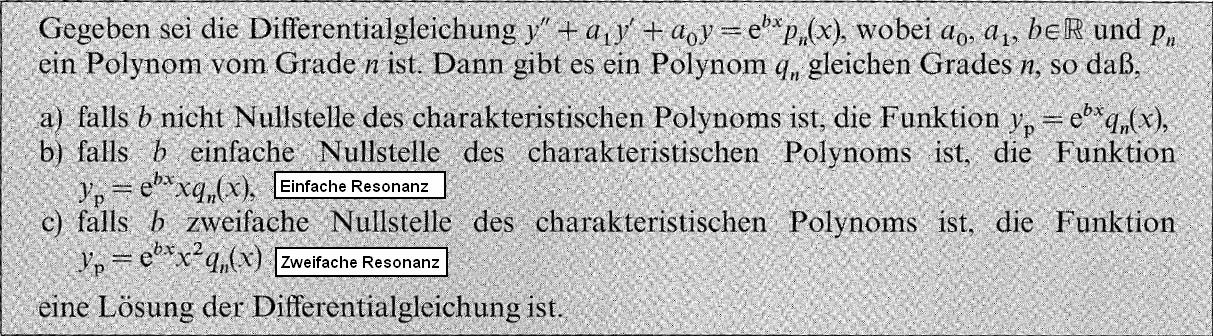
\includegraphics[width=\linewidth]{images/DGL_Part_2.jpg}
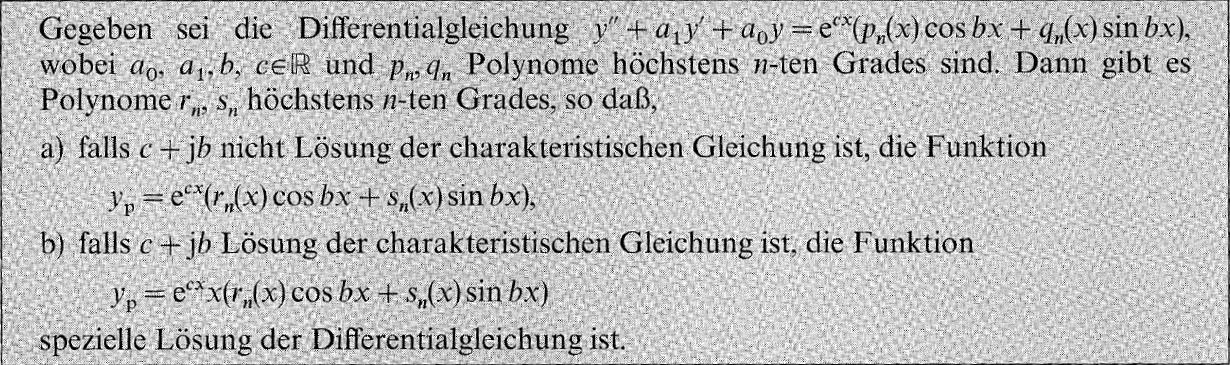
\includegraphics[width=\linewidth]{images/DGL_Part_3.jpg}
\clearpage
\pagebreak

\subsection{Integralgesetze}
\subsubsection{Der Satz von Gauss}
Das Volumenintegral über die Divergenz eines Vektorfeldes wird in ein Oberflächenintegral umgewandelt.\\
$\boxed{\int\limits_V \divergenz \vec F dv = \oint\limits_{\partial V} \vec F \cdot \vec{dA}}$
\subsubsection{Der Satz von Stokes}
Das Oberflächenintegral über die Rotation eines Vektorfeldes wird in ein Kurvenintegral umgewandelt. \\
$\boxed{\int\limits_A \rotation \vec{F}\cdot d\vec{A}  = \oint\limits_{\partial A}\vec{F}\cdot d\vec{s}}$
\subsubsection{Der Satz von Green}
Die Greensche Formel beschreibt den Zusammenhang zwischen Wegintegral und einem Oberflächenintegral.\\
$\boxed{\int\limits_A \frac{\partial F_2}{\partial x} - \frac{\partial F_1}{\partial y} dA = \oint\limits_{\partial A}\vec{F}\cdot d\vec{s}}$
\subsection{Weiteres}
Die Bedeutung der nachfolgenden Integralgleichungen ist die fundamentale Grundlage elektromagnetische Feldtheorie. Der elektrische Strom erzeugt das elektrische Feld in seiner Umgebung (Gausssches Gesetz), der elektrische Strom erzeugt das quellenfreie rotationssymmetrische magnetische Feld (Coulombsches Gesetz), die Verteilung des magnetischen Feldes durch eine geschlossene Kurve ist der gesamte Strom durch die entsprechende Fläche (Ampèresches Gesetz) und das zeitvariante magnetische Feld induziert eine elektrische Spannung (Faradaysches Gesetz).\\
Durch die Gesetze von Stokes und Gauss können diese 4 Gesetze in die Maxwellgleichungen überführt werden. 
\vspace{-0.8cm}
\begin{longtable}{p{.30\textwidth} p{.65\textwidth}}
	\textbf{Elektrostatik} & Die Elektrostatik befasst sich mit ruhenden elektrischen Ladungen, Ladungsverteilungen und den elektrischen Feldern geladener Körper
	Die Phänomene der Elektrostatik rühren von den Kräften her, die elektrische Ladungen aufeinander ausüben. Diese Kräfte werden vom coulombschen Gesetz beschrieben.\\
	\textbf{Elektrodynamik} & Die Elektrodynamik befasst sich mit bewegten elektrischen Ladungen und mit zeitlich veränderlichen elektrischen und magnetischen Feldern. Diese Vorgänge werden durch die Maxwellgleichungen beschrieben. \\
\end{longtable}
\subsection{Einheiten}
\renewcommand{\arraystretch}{1.5}
\begin{tabular}{|p{3.5cm}|p{1.5cm}|p{3cm}||p{3.5cm}|p{1.5cm}|p{3.2cm}|}
	\hline
	\textbf{Name}			&\textbf{Zeichen} & \textbf{Einheit}&
	\textbf{Name}			&\textbf{Zeichen} & \textbf{Einheit}\\
	\hline
	\textbf{Elektr. Feld} 	& $\vec{E}$	& $[E] = \frac{V}{m}$&	
	\textbf{Magn. Feld}		& $\vec{H}$ & $[H] = \frac{A}{m}$\\
	\hline
	\textbf{Elektr. Flussdichte}&$\vec{D}$&$[D] = \frac{C}{m^2}$&
	\textbf{Magn. Flussdichte}&$\vec{B}$&$[B] = \frac{Vs}{m^2}=T$\\
	\hline
	\textbf{Elektr. Stromdichte} &$\vec{J}$& $[J]=\frac{A}{m^2}$&
	\textbf{Elektr. Widerstand} &$R$ &$[R]=\Omega$\\
	\hline
	\textbf{Spannung}&$U$&$[U]=V$&
	\textbf{Strom}&$I$&$[I]=A$\\
	\hline
	\textbf{Induktivität}&$L$&$[L]=\frac{Vs}{A}=H$&
	\textbf{Magn. Spannung}&$V_{m}=\Theta$&$[V_{m}]=A$\\
	\hline
	\textbf{Kapazität}&$C$&$[C]=F$&
	\textbf{Magn. Fluss}&$\phi$&$[\phi]=Wb=Vs$\\
	\hline
	\textbf{Permeabilität}&$\mu_{0} $&$[\mu_{0}]=4\pi 10^{-7}$&
	\textbf{Permittivität}&$\epsilon_{0}$&$[\epsilon_{0}]=8.854\cdot 10^{-12}$\\
	\hline
	\textbf{Spez. Leitfähigkeit}&$\sigma$&$[\sigma]=\frac{S}{m}$&
	\textbf{Spez. Widerstand}&$\rho $&$[\rho]=\Omega m $\\
	\hline
\end{tabular}

\clearpage
\pagebreak